% KEYSTONE: Journal of Computer Security submission (anonymized main manuscript).
% Built with Sage's sagej.cls (Crown trim, Vancouver/numbered citations).
% All result numbers are generated macros from ../r1/tables/numbers.tex and the
% tables are the generated files in ../r1/tables, so text and data cannot drift.
\documentclass[Crown,sagev]{sagej}

\usepackage{booktabs}
\usepackage{array}
\usepackage{tabularx}
\usepackage{enumitem}
\usepackage{xcolor}
\usepackage[font=small,labelfont=bf]{caption}
\usepackage{subcaption}
\usepackage{url}
\usepackage[hidelinks]{hyperref}
\hypersetup{pdftitle={KEYSTONE: Readiness Audits for Dispute-Key Availability in Encrypted Rollups},pdfauthor={},pdfkeywords={dispute-key availability, threshold decryption, encrypted rollups, readiness audit}}
\renewcommand{\topfraction}{0.9}
\renewcommand{\bottomfraction}{0.8}
\renewcommand{\textfraction}{0.07}
\renewcommand{\floatpagefraction}{0.8}
\setcounter{topnumber}{3}
\setcounter{totalnumber}{5}

\graphicspath{{figures/}{../r1/figures/}}
\setlist{nosep,leftmargin=*}

\theoremstyle{plain}
\newtheorem{theorem}{Theorem}
\newtheorem{lemma}{Lemma}
\newtheorem{proposition}{Proposition}
\newtheorem{corollary}{Corollary}
\newtheorem{observation}{Observation}
\theoremstyle{definition}
\newtheorem{definition}{Definition}
\newtheorem{assumption}{Assumption}
\theoremstyle{remark}
\newtheorem{remark}{Remark}

\newcommand{\DKA}{\mathrm{DKA}}
\newcommand{\CA}{\mathrm{CA}}
\newcommand{\VSR}{\mathrm{VSR}}
\newcommand{\AKR}{\mathrm{AKR}}
\newcommand{\AD}{\mathrm{AD}}
\newcommand{\DDL}{\mathrm{DDL}}
\newcommand{\PAC}{\mathrm{PAC}}
\newcommand{\Ready}{\mathsf{Ready}}
\newcommand{\G}{\mathbb{G}}
\newcommand{\Zq}{\mathbb{Z}_\ell}

\newcommand{\RIIDAudit}{43.1\%}
\newcommand{\RIIDRecon}{99.98\%}
\newcommand{\RStratDetU}{99.89\%}
\newcommand{\RStratDetS}{100.00\%}
\newcommand{\RStratPassU}{37.3\%}
\newcommand{\RStratPassS}{34.9\%}
\newcommand{\RStratD}{0.00021}
\newcommand{\RStratHW}{0.0075}
\newcommand{\RStratDiscordant}{28}
\newcommand{\RSWAudit}{100.0\%}
\newcommand{\RSWDispute}{0.0\%}
\newcommand{\RSWDisputeHi}{0.0029\%}
\newcommand{\RAccEightSevenDet}{85.9\%}
\newcommand{\RAccEightSevenPass}{81.3\%}
\newcommand{\RAccSixteenFourteenDet}{98.8\%}
\newcommand{\RAccSixteenFourteenPassFive}{95.7\%}
\newcommand{\RAccSixteenFourteenPassTen}{78.9\%}
\newcommand{\RDomTwoRecon}{81.0\%}
\newcommand{\RDomFourRecon}{94.8\%}
\newcommand{\RIIDReconTen}{99.98\%}
\newcommand{\RProveTwoK}{130.3}
\newcommand{\RVerifyTwoK}{135.4}
\newcommand{\RCombineTwoK}{3213}
\newcommand{\RCombineThreeK}{10201}
\newcommand{\RDLControlMed}{3818}
\newcommand{\RDLControlPninefive}{3936}
\newcommand{\RDLControlByHalf}{0.0\%}
\newcommand{\RDLControlByOne}{0.0\%}
\newcommand{\RDLControlByTwo}{0.0\%}
\newcommand{\RDLControlByFive}{99.7\%}
\newcommand{\RDLControlAudit}{100.0\%}
\newcommand{\RDLControlSucc}{299/300}
\newcommand{\RDLRegionalMed}{3841}
\newcommand{\RDLRegionalPninefive}{3908}
\newcommand{\RDLRegionalByHalf}{0.0\%}
\newcommand{\RDLRegionalByOne}{0.0\%}
\newcommand{\RDLRegionalByTwo}{0.0\%}
\newcommand{\RDLRegionalByFive}{100.0\%}
\newcommand{\RDLRegionalAudit}{100.0\%}
\newcommand{\RDLRegionalSucc}{300/300}
\newcommand{\RDLGlobalMed}{3875}
\newcommand{\RDLGlobalPninefive}{4016}
\newcommand{\RDLGlobalByHalf}{0.0\%}
\newcommand{\RDLGlobalByOne}{0.0\%}
\newcommand{\RDLGlobalByTwo}{0.0\%}
\newcommand{\RDLGlobalByFive}{100.0\%}
\newcommand{\RDLGlobalAudit}{100.0\%}
\newcommand{\RDLGlobalSucc}{300/300}
\newcommand{\RDLLossMed}{3829}
\newcommand{\RDLLossPninefive}{3886}
\newcommand{\RDLLossByHalf}{0.0\%}
\newcommand{\RDLLossByOne}{0.0\%}
\newcommand{\RDLLossByTwo}{0.0\%}
\newcommand{\RDLLossByFive}{100.0\%}
\newcommand{\RDLLossAudit}{71.7\%}
\newcommand{\RDLLossSucc}{300/300}
\newcommand{\RDLCrashTenMed}{3692}
\newcommand{\RDLCrashTenPninefive}{3775}
\newcommand{\RDLCrashTenByHalf}{0.0\%}
\newcommand{\RDLCrashTenByOne}{0.0\%}
\newcommand{\RDLCrashTenByTwo}{0.0\%}
\newcommand{\RDLCrashTenByFive}{100.0\%}
\newcommand{\RDLCrashTenAudit}{2.3\%}
\newcommand{\RDLCrashTenSucc}{300/300}
\newcommand{\RDLCrashElevenMed}{--}
\newcommand{\RDLCrashElevenPninefive}{--}
\newcommand{\RDLCrashElevenByHalf}{0.0\%}
\newcommand{\RDLCrashElevenByOne}{0.0\%}
\newcommand{\RDLCrashElevenByTwo}{0.0\%}
\newcommand{\RDLCrashElevenByFive}{0.0\%}
\newcommand{\RDLCrashElevenAudit}{1.7\%}
\newcommand{\RDLCrashElevenSucc}{0/300}
\newcommand{\RDLDomainOutMed}{3700}
\newcommand{\RDLDomainOutPninefive}{3780}
\newcommand{\RDLDomainOutByHalf}{0.0\%}
\newcommand{\RDLDomainOutByOne}{0.0\%}
\newcommand{\RDLDomainOutByTwo}{0.0\%}
\newcommand{\RDLDomainOutByFive}{100.0\%}
\newcommand{\RDLDomainOutAudit}{5.7\%}
\newcommand{\RDLDomainOutSucc}{300/300}
\newcommand{\RDLHeavyTailMed}{3772}
\newcommand{\RDLHeavyTailPninefive}{3850}
\newcommand{\RDLHeavyTailByHalf}{0.0\%}
\newcommand{\RDLHeavyTailByOne}{0.0\%}
\newcommand{\RDLHeavyTailByTwo}{0.0\%}
\newcommand{\RDLHeavyTailByFive}{100.0\%}
\newcommand{\RDLHeavyTailAudit}{98.3\%}
\newcommand{\RDLHeavyTailSucc}{300/300}
\newcommand{\RDLTraces}{300}
\newcommand{\RExpLoss}{72.4\%}
\newcommand{\RExpCrashTen}{3.0\%}
\newcommand{\RExpDomainOut}{7.0\%}
\newcommand{\RDLAuditMedLo}{1.24}
\newcommand{\RDLAuditMedHi}{1.43}
\newcommand{\RDLMedLo}{3.69}
\newcommand{\RDLMedHi}{3.88}
\newcommand{\RDLMaxSucc}{4.48}

\newcommand{\OcEightTwentyOne}{1.9\%}
\newcommand{\OcEightTwentyTwo}{3.0\%}
\newcommand{\OcEightTwentySix}{14.9\%}
\newcommand{\SepSFour}{25}
\newcommand{\SepQFour}{19}
\newcommand{\SepSSix}{20}
\newcommand{\SepQSix}{16}
\newcommand{\SepSEight}{14}
\newcommand{\SepQEight}{12}
\newcommand{\AsnEightDead}{9.8}
\newcommand{\AsnEightLive}{4.6}
\newcommand{\AsnSixteenDead}{2.3}
\newcommand{\AsnSixteenLive}{1.1}
\newcommand{\McNemarP}{7.5\times10^{-9}}


\begin{document}
\setcounter{secnumdepth}{3}
\pdfinfoomitdate=1
\pdftrailerid{}

\runninghead{Readiness audits for dispute-key availability}

\title{KEYSTONE: Readiness Audits for Dispute-Key Availability in Encrypted Rollups}

\author{[Author details removed for peer review]}

\begin{abstract}
Encrypted optimistic rollups can keep ciphertexts and execution receipts available and still fail a dispute because the threshold service that must decrypt the disputed record is unavailable, late or uncooperative. We call the missing property dispute-key availability (DKA) and separate it from ciphertext availability, valid-share registration, audit-time readiness, authorized decryptability and deadline liveness. KEYSTONE audits readiness with sampled canary shares, in the style of threshold-coin shares, carrying Chaum--Pedersen proofs; their transcripts are simulatable from public shares, so audits exercise real shares without revealing any record. We give exact operating characteristics for uniform and stratified samples, a placement condition and a deadline budget. We show that a single small audit cannot separate a committee one share short of its threshold from a live one, whereas a sequential test across audits can, and that confidentiality against parties who obtain other records' releases requires binding each release to its record. Exact analysis, simulation and a single-host 32-process testbed with ffdhe2048 cryptography confirm these separations, show that selective withholders pass every audit while defeating every dispute, and show that serial proof verification bounded completion time in our unoptimized prototype.
\end{abstract}

\keywords{Dispute-key availability, threshold decryption, encrypted rollups, readiness audit, acceptance sampling, selective withholding}

\maketitle

% =====================================================================
\section{Introduction}\label{sec:intro}

Optimistic rollups execute transactions off chain and accept the result unless a challenger proves it wrong within a dispute window\cite{kalodner2018arbitrum}. When the executed workload is private, as in encrypted machine-learning inference\cite{conway2024opml,eigenai2026}, the records a challenger needs are published only as ciphertexts. Data-availability mechanisms can keep these ciphertexts retrievable. They cannot ensure that the committee holding shares of the decryption key delivers enough valid decryption contributions once a dispute is authorized and before its deadline. A ciphertext that cannot be opened in time is, for the dispute, unavailable. We use AI-rollup disputes as a running example, but nothing in our model depends on the workload: the same question arises wherever a protocol must open threshold-encrypted inputs on demand.

The failure is silent until it is needed. Custodians may lose shares, fail together when a provider or region goes down, or run broken software, and the key must stay serviceable for a dispute window that lasts days and may outlive the committee that sealed the record. A strategic custodian may also answer every routine check and refuse one targeted dispute; we show that no audit of the kind studied here can detect that, and treat it as a limit rather than a goal. Existing building blocks answer adjacent questions: threshold encryption limits who can decrypt\cite{desmedt1990threshold}, verifiable secret sharing shows that shares were distributed correctly\cite{feldman1987vss,schoenmakers1999pvss}, proactive sharing refreshes them\cite{herzberg1995proactive}, and proofs of retrievability and data-availability sampling check that data can be retrieved\cite{juels2007por,albassam2021fraud}. None produces public evidence that enough custodians can serve an authorized dispute now, or states what such evidence implies.

In this article, we study this property, \emph{dispute-key availability} (DKA), and we design and evaluate KEYSTONE, a readiness audit for it that targets non-strategic faults. KEYSTONE seals each record under a fresh key wrapped by a threshold Diffie--Hellman KEM. Routine audits ask a beacon-sampled subset of custodians to apply their shares to a \emph{canary}, a group element hashed from public audit context, and to prove correctness with a Chaum--Pedersen equality-of-discrete-logarithm (DLEQ) proof; each response is structurally a threshold-coin or threshold-signature share on a hashed message\cite{cachin2005constantinople,boldyreva2003threshold}. An authorized dispute applies the same share operation to the disputed record under a public request-and-deadline transcript. Our contributions are:
\begin{enumerate}
  \item \textbf{A property decomposition} (Section~\ref{sec:properties}): definitions of ciphertext availability, valid-share registration, audit-time readiness, authorized decryptability, deadline liveness, pre-authorization confidentiality and $(\varepsilon,\Delta_d)$-DKA, with constructive witnesses for three inferences a deployment must not draw.
  \item \textbf{A confidentiality-preserving audit} (Section~\ref{sec:protocol}): we use threshold-coin-style shares as a sampled readiness test; adapting the standard simulation argument, canary transcripts are simulatable from public shares in the random-oracle model, and a coordinator cannot substitute a production record for a canary. We also show that the plain threshold KEM is malleable across records, so confidentiality against parties who obtain other records' releases requires binding each release to its record.
  \item \textbf{An exact analysis} (Section~\ref{sec:analysis}): full operating characteristics for uniform and stratified samples, showing that small audits cannot separate a committee one share short of $t$ from a live one, the sample sizes and sequential tests that certify a stated safety margin, a placement condition, the detection versus benign-alarm trade-off, and a deadline budget.
  \item \textbf{An evaluation with labeled evidence} (Section~\ref{sec:evaluation}) that combines exact analysis, three prespecified simulation cells, microbenchmarks at RFC~7919 group sizes and a 32-custodian emulated testbed, and reports negative results: a high benign alarm rate under the strictest rule, a selective-withholding counterexample and a primary deadline endpoint that no profile met.
\end{enumerate}
None of the primitives is new, and a passed audit does not prove future availability.

Sections~\ref{sec:prelim}--\ref{sec:evaluation} cover preliminaries, model, properties, protocol, analysis and evaluation; Sections~\ref{sec:discussion}--\ref{sec:conclusion} cover design consequences, related work, limitations and conclusions.

% =====================================================================
\section{Preliminaries}\label{sec:prelim}

\paragraph{Groups and sharing.} Let $\G$ be a cyclic group of prime order $\ell$ with generator $g$ in which the decisional Diffie--Hellman (DDH) problem is hard. The prototype uses the order-$\ell$ subgroup of quadratic residues modulo the RFC~7919 safe primes\cite{rfc7919} (ffdhe2048, ffdhe3072), with $\ell=(p-1)/2$ and $g=4$; $q$ denotes only the acceptance threshold of an audit, and $\binom{a}{b}=0$ when $b>a$ or $b<0$. A secret $x\in\Zq$ is Shamir-shared with a polynomial $f$ of degree $t-1$, $f(0)=x$; custodian $i\in\{1,\dots,n\}$ holds $x_i=f(i)$ and publishes $Y_i=g^{x_i}$\cite{shamir1979share}, verifiable against Feldman commitments\cite{feldman1987vss}. Any $t$ distinct indices $I$ have Lagrange coefficients $\lambda_i^I$ with $\sum_{i\in I}\lambda_i^I x_i=x$.

\paragraph{Threshold Diffie--Hellman KEM.} With epoch key $PK=g^{x}$, a sender draws $\rho\leftarrow\Zq$, publishes $C_1=g^{\rho}$ and derives a key-encryption key from $PK^{\rho}$ and the record identifier. Any $t$ partial decryptions $C_1^{x_i}$ determine $C_1^{x}=\prod_{i\in I}(C_1^{x_i})^{\lambda_i^I}$. This threshold ElGamal KEM\cite{desmedt1990threshold} is semantically secure under DDH in the random-oracle model but malleable: anyone can turn $C_1$ into $C_1g^{\gamma}$. Shoup and Gennaro's TDH2 binds a label and a proof of knowledge of $\rho$ to the ciphertext, which makes it secure against chosen-ciphertext attacks\cite{shoup2002securing}; Section~\ref{sec:conf} explains when KEYSTONE needs it.

\paragraph{DLEQ proofs, hashing and beacon.} A Chaum--Pedersen proof\cite{chaum1992dleq} shows $\log_g Y_i=\log_X D_i$: the prover picks $\nu\leftarrow\Zq$, sends $a_1=g^{\nu}$, $a_2=X^{\nu}$, derives $c=H(g,Y_i,X,D_i,a_1,a_2,\mathsf{ctx})$ by the Fiat--Shamir transform\cite{fiat1987prove} and returns $z=\nu+c\,x_i$; the verifier checks $g^{z}=a_1Y_i^{c}$ and $X^{z}=a_2D_i^{c}$. The protocol is complete, special-sound and honest-verifier zero knowledge, and the request context $\mathsf{ctx}$ ties each proof to one request. $H_G$ maps byte strings to $\G\setminus\{1\}$ with domain separation; we model $H$ and $H_G$ as random oracles. A public beacon outputs values that are unpredictable before publication\cite{das2022spurt}.

% =====================================================================
\section{System and threat model}\label{sec:model}

An epoch $E$ has $n$ custodians placed in failure domains (providers, regions, software stacks), a threshold $t$, a key $PK_E$ and registered public shares $Y_1,\dots,Y_n$. A rollup worker encrypts each inference record $r$ under a fresh data key $K_r$ with AES-GCM, wraps $K_r$ under the KEM key derived from $(C_1^{(r)},PK_E)$, and publishes the result to a data-availability (DA) layer. A settlement layer, the \emph{bulletin board}, records registrations, requests, deadlines and evidence and supplies an ordered public clock. A \emph{combiner} inside the authorized destination collects partial decryptions; it learns $K_r$ for records it is authorized to open and is trusted not to disclose it. Dispute partials reach it over authenticated, confidential channels, and the board stores only commitments to responses with their validity status and timestamps, so it never holds enough material to decrypt a record. Canary responses may be public (Lemma~\ref{lem:sim}). Figure~\ref{fig:architecture} shows the three paths.

\begin{figure}[t]
\centering
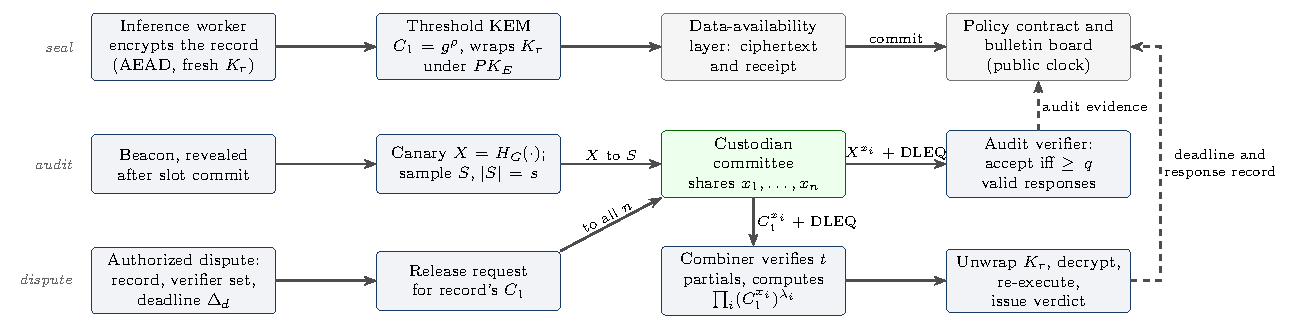
\includegraphics[width=\textwidth]{fig1_architecture.pdf}
\caption{KEYSTONE architecture. Sealing, routine canary auditing and authorized dispute release are separate paths over one custodian committee. The audit uses a beacon-derived canary, never a production ciphertext; only an authorized dispute requests partial decryptions of a record's KEM component $C_1$. Dashed arrows are public evidence written to the bulletin board.}
\label{fig:architecture}
\end{figure}

\begin{assumption}[Threshold confidentiality]\label{as:conf}
During an epoch the adversary learns fewer than $t$ current shares. DDH is hard in $\G$; $H$, $H_G$ and the key-derivation function are independent, domain-separated random oracles; and AES-GCM is a secure authenticated-encryption scheme.
\end{assumption}

\begin{assumption}[Beacon]\label{as:beacon}
An audit's beacon value is unpredictable until its epoch, slot and committee are committed on the bulletin board, and the derived sample is uniform (without replacement, or within each domain quota for stratified samples) and independent of other audits' samples. The prototype seeds a pseudorandom generator with a SHA-256 hash of the beacon; we model this as ideal, and a production system should use a cryptographic sampler.
\end{assumption}

\begin{assumption}[Bulletin board and data availability]\label{as:board}
The bulletin board is append-only and totally ordered and exposes each request to custodians within $\delta_b$. The DA layer keeps committed ciphertexts and receipts retrievable.
\end{assumption}

\begin{assumption}[Bounded delay, for deadline statements only]\label{as:sync}
Messages between non-faulty parties arrive within $\delta$ over channels that authenticate the sending custodian. A non-faulty custodian produces a partial decryption with proof within $c_p$; the combiner verifies one proof within $c_v$ and combines $t$ partials within $c_c$.
\end{assumption}

Detection and confidentiality statements do not use Assumption~\ref{as:sync}. The adversary may crash custodians individually or by domain, cause share loss, send invalid or equivocal responses, move corruption across epochs, issue unauthorized requests, act as a worker that commits records of its choice and obtains disputes on them, and control \emph{selective} custodians that answer canaries but withhold targeted dispute responses. Corruption is static within an epoch: the adversary fixes the custodians it controls when the epoch starts. Out of scope are production key-generation security, malicious combiners, verifiers or trusted execution environments that leak records they are authorized to open, arbitrary asynchronous partitions, and selective withholding beyond the counterexample of Observation~\ref{prop:nonimpl}. Two limits follow from the model. An audit shows that whoever answered knows $x_i$, not that the registered operator does, so share pooling by one operator and false failure-domain declarations are invisible to it. And threshold custody replaces the one-honest-challenger assumption of optimistic rollups with an assumption on $t$ of $n$ custodians.

% =====================================================================
\section{Dispute-key availability}\label{sec:properties}

Fix an epoch $E$, a record $r$ with KEM component $C_1$, and a request time $\tau$ on the bulletin board.

\begin{definition}[Ciphertext availability]\label{def:ca}
$\CA(r,\tau)$ holds if the committed encrypted record and its receipt are retrievable from the DA layer at $\tau$.
\end{definition}

\begin{definition}[Valid-share registration]\label{def:vsr}
$\VSR(E)$ holds if the registered public shares are consistent with one degree-$(t-1)$ polynomial whose constant term is the epoch secret, and every admitted custodian initially received the matching share.
\end{definition}

\begin{definition}[Readiness]\label{def:ready}
For a request $u$, an audit or a dispute on a named record, $\Ready_i(E,\tau,u,\Delta)=1$ if custodian $i$ can access its current share, perform the operation $u$ requests, produce a valid DLEQ proof and deliver the response by $\tau+\Delta$. Audit readiness and dispute readiness for each record are distinct predicates.
\end{definition}

\begin{definition}[Audit-time readiness]\label{def:akr}
For a sample $S$ of $s$ custodians and threshold $q\le s$, $\AKR(E,S,\tau)$ holds if at least $q$ members of $S$ deliver valid canary responses by the audit deadline.
\end{definition}

\begin{definition}[Authorized decryptability and deadline liveness]\label{def:ad}
After a valid authorization for $r$ at $\tau$, $\AD(r,E,\tau)$ holds if the combiner obtains valid partial decryptions of $C_1$ from at least $t$ distinct custodians, and $\DDL(r,E,\tau,\Delta_d)$ holds if this happens by $\tau+\Delta_d$.
\end{definition}

\begin{definition}[Pre-authorization confidentiality]\label{def:pac}
$\PAC$ holds for $r$ if no probabilistic polynomial-time adversary that satisfies Assumption~\ref{as:conf} and observes all audit transcripts, but no dispute releases, distinguishes $K_r$ from a random key with non-negligible advantage. In the stronger $\PAC^{+}$, the adversary may also commit records of its choice and obtain the release of every record other than $r$, where a \emph{release} is the set of partial decryptions and the combined value delivered to the authorized destination, which the adversary may control for its own records.
\end{definition}

\begin{definition}[Dispute-key availability]\label{def:dka}
Fix a readiness model, a distribution over custodian failures, share loss and message delays over time. An epoch provides $(\varepsilon,\Delta_d)$-$\DKA$ under it if for every committed record $r$ and authorization time $\tau$, $\Pr[\DDL(r,E,\tau,\Delta_d)]\ge 1-\varepsilon$ over the readiness model and the protocol's randomness, and $\PAC$ holds for every record before its authorization.
\end{definition}

\begin{definition}[Catastrophic state and detection]\label{def:fa}
An epoch is \emph{catastrophic} at $\tau$ if fewer than $t$ custodians are audit-ready. An audit \emph{falsely accepts} if $\AKR$ holds in a catastrophic state; its \emph{detection probability} is one minus its false-accept probability. Dispute readiness can be lower than audit readiness (Observation~\ref{prop:nonimpl}).
\end{definition}

\begin{remark}[Timescale and epochs]
Deployed optimistic rollups keep dispute windows open for days and bound each interactive move by hours, so DKA chiefly requires the key to stay serviceable throughout the window ($\varepsilon$ over the window), while $\Delta_d$ matters for per-move timers and short-window designs. A record sealed under $PK_E$ remains disputable after the committee of $E$ rotates, so DKA must hold across epochs: old committees stay serviceable until their records' windows close, or shares are handed over by dynamic proactive sharing\cite{maram2019churp,yurek2023dpss}, and audits must cover every epoch with open records.
\end{remark}

DKA is conditional and probabilistic. The next observation records what the weaker properties do not imply. Its witnesses are elementary; each blocks a tempting inference, and the design is organized around them.

\begin{observation}[Non-implications]\label{prop:nonimpl}
Fix $1\le t\le n$, $1\le q\le s\le n$ and $\Delta_d$.
\begin{enumerate}
  \item $\CA(r,\tau)$ does not imply $\DDL(r,E,\tau,\Delta_d)$.
  \item $\AKR(E,S,\tau)$ does not imply $\AD(r,E,\tau')$ for an authorized dispute at $\tau'\ge\tau$.
  \item For every $m$, $m$ accepted audits at times $\tau_1<\dots<\tau_m$ do not imply $\AD(r,E,\tau')$ for $\tau'>\tau_m$.
\end{enumerate}
\end{observation}

\begin{proof}
(1) Let the DA layer retain the record while exactly $t-1$ custodians are dispute-ready for $r$ and the others have lost their shares. $\CA$ holds, but at most $t-1$ valid partials exist, so $\AD$ and $\DDL$ fail.
(2) Let all custodians be audit-ready and let $w=n-t+1$ of them answer every canary and withhold every response for $r$. Every sample has $s\ge q$ valid responses, so $\AKR$ holds for every $S$, while at most $t-1$ custodians answer the dispute.
(3) Take two executions identical up to $\tau_m$ with all custodians audit-ready, so all $m$ audits accept in both. Afterwards all custodians stay ready in the first and $n-t+1$ lose their shares in the second. The audit histories are identical but $\AD$ holds at $\tau'$ only in the first, so without assumptions on how readiness evolves no predicate of the audit history implies $\AD$ at $\tau'$; Corollary~\ref{cor:repeat} shows what a static model recovers.
\end{proof}

Item~(2) is why audit and dispute readiness are separate predicates; item~(3) is why any repeated-audit guarantee needs a temporal model.

% =====================================================================
\section{The KEYSTONE protocol}\label{sec:protocol}

\paragraph{Setup and sealing.} The committee is formed under identity, stake and failure-domain placement policy (Observation~\ref{prop:cap}). A deployment would use an authenticated distributed key generation or publicly verifiable secret sharing\cite{gennaro2007dkg,das2022adkg,schoenmakers1999pvss}; the prototype uses a dealer with Feldman commitments as an explicit substitution boundary. To seal $r$, the worker draws $\rho$, computes $C_1=g^{\rho}$ and $\kappa=\mathrm{KDF}(PK_E^{\rho},\mathsf{id}_r,\mathsf{aad})$, wraps $K_r$ under $\kappa$, encrypts the record under $K_r$ with AES-GCM, and publishes an envelope binding epoch, record identifier, ciphertext, metadata and DA pointer.

\paragraph{Readiness audit.} The coordinator commits an epoch and audit slot. The next finalized beacon value $\beta$ fixes a sample $S$ of $s$ custodians, uniform or stratified by domain, and everyone derives the canary $X=H_G(\texttt{KEYSTONE-CANARY}\parallel E\parallel \mathsf{slot}\parallel \beta)$. Each sampled custodian returns $D_i=X^{x_i}$ with a DLEQ proof that $\log_g Y_i=\log_X D_i$, bound to the request context and its index. The verifier checks membership, freshness, uniqueness per index, proof validity and the deadline, and accepts after $q$ valid responses.

\paragraph{Authorized dispute.} A dispute starts once the policy contract binds a record, epoch, authorized verifier and deadline $\Delta_d$. Each custodian checks the authorization and returns $C_1^{x_i}$ with a DLEQ proof bound to the dispute. The combiner verifies responses on arrival, discards duplicates and invalid ones, stops at $t$ valid partials, interpolates $C_1^{x}=PK_E^{\rho}$, re-derives $\kappa$, unwraps $K_r$ and decrypts.

\paragraph{Transcript and evidence.} For each request, the board records commitments to valid, invalid, equivocal, stale and unauthorized responses and the absence of missing ones, with timestamps. Invalid proofs and conflicting responses are self-contained cryptographic evidence; attributing a missing response to a custodian additionally requires Assumption~\ref{as:sync}. The prototype contract is a skeleton: an administrator supplies the sample and canary hash when opening an audit without an on-chain beacon check, records invalid-response evidence after off-chain verification, and can cancel requests. Theorem~\ref{thm:fa} therefore holds for the prototype only if the administrator samples as the protocol prescribes; deriving the sample on chain from the committed beacon and verifying proofs on chain are needed for a trustless deployment.

\subsection{Security of the audit}

\begin{lemma}[Correctness and knowledge soundness]\label{lem:correct}
An honest response passes verification. In the random-oracle model a verifying response satisfies $D_i=X^{x_i}$ except with negligible probability, and the proof is a proof of knowledge: from any party that produces verifying responses for fresh canaries with non-negligible probability, an extractor obtains $x_i$. Any $t$ verified partials of $C_1$ with distinct indices $I$ combine to $\prod_{i\in I}(C_1^{x_i})^{\lambda_i^I}=PK_E^{\rho}$.
\end{lemma}

\begin{proof}
Completeness: $g^{z}=g^{\nu+cx_i}=a_1Y_i^{c}$ and $X^{z}=a_2D_i^{c}$ when $D_i=X^{x_i}$. The protocol is special-sound, since two accepting transcripts with one commitment and different challenges yield $x_i$; with the Fiat--Shamir hash as a random oracle, the forking lemma turns a party that succeeds with non-negligible probability into an extractor, and value soundness follows\cite{chaum1992dleq,fiat1987prove}. Combination: $\prod_{i\in I}C_1^{x_i\lambda_i^I}=C_1^{x}=g^{\rho x}=PK_E^{\rho}$.
\end{proof}

Knowledge soundness makes a passed audit meaningful: whoever passes canary audits with non-negligible probability holds $x_i$, and under Assumption~\ref{as:conf} the adversary cannot obtain an honest custodian's share from public values without solving a discrete logarithm.

\begin{lemma}[Audit transcripts are simulatable]\label{lem:sim}
Model $H_G$ and $H$ as random oracles. A simulator that knows only $g$ and $Y_1,\dots,Y_n$ answers all queries to $H_G$ and $H$ and produces the honest custodians' audit responses $(X,(D_i,\pi_i)_{i\in S})$ for any audit context and any $S$, including $S=\{1,\dots,n\}$. With at most $N$ simulated proofs and $Q$ oracle queries, simulated and real views are within statistical distance $NQ/\ell$, so observing audits changes any adversary's advantage against $\PAC$, measured as $|\Pr[1\mid K_r]-\Pr[1\mid\text{random}]|$, by at most $2NQ/\ell$.
\end{lemma}

\begin{proof}
The simulator answers every fresh $H_G$ query, from the protocol or the adversary, with $g^{a}$ for a stored $a\leftarrow\mathbb{Z}_\ell^{*}$, which is exactly a random oracle onto $\G\setminus\{1\}$. For an honest custodian and canary $X=g^{a}$ it sets $D_i=Y_i^{a}=X^{x_i}$, the real response. Each proof is produced by the honest-verifier zero-knowledge simulator: draw $c,z\leftarrow\Zq$, set $a_1=g^{z}Y_i^{-c}$ and $a_2=X^{z}D_i^{-c}$, and program $H$ at that input to $c$. Since $a_1$ is uniform, the input was queried before with probability at most $Q/\ell$, and a union bound over $N$ proofs gives the distance. Corrupted custodians' responses come from the adversary. Because $H$, $H_G$ and the key-derivation function are independent and domain separated, this programming does not interfere with a reduction to the KEM that programs the key-derivation oracle, so an adversary against $\PAC$ that sees audits becomes one against the threshold KEM alone, each output probability moving by at most $NQ/\ell$.
\end{proof}

This is the standard simulation argument for threshold-coin and threshold-signature shares on hashed messages\cite{cachin2005constantinople,boldyreva2003threshold}, which we restate for the audit setting. Lemma~\ref{lem:sim} holds even for adversarially chosen audit contexts and beacons. It is why the audit can exercise every sampled share without opening any record: combining $t$ canary partials yields $X^{x}$ for a hash-derived $X$, which equals a fixed record component only with negligible probability.

\begin{lemma}[No production substitution]\label{lem:subst}
Model $H_G$ as a random oracle. For a fixed $C_1$, a coordinator making $Q$ queries to $H_G$ finds an audit context whose canary equals $C_1$ with probability at most $Q/(\ell-1)$.
\end{lemma}

\begin{proof}
Each query returns an independent uniform element of $\G\setminus\{1\}$, equal to the fixed $C_1\neq1$ with probability $1/(\ell-1)$; apply the union bound.
\end{proof}

\begin{remark}
The prototype hashes to an integer modulo $p$ and squares into the quadratic residues; a production system should use a standardized hash-to-curve suite\cite{rfc9380}. Binding request context into the Fiat--Shamir hash gives verification-domain binding, not the share isolation of context-dependent threshold decryption\cite{boneh2025context}. The lemmas do not cover side channels.
\end{remark}

\subsection{Confidentiality against releases of other records}\label{sec:conf}

Lemma~\ref{lem:sim} concerns audits only. An adversary that can also obtain releases, for example a worker that commits and disputes its own records, defeats the plain KEM.

\begin{proposition}[Malleability across records]\label{prop:malleable}
With the plain threshold Diffie--Hellman KEM, $\PAC^{+}$ does not hold: an adversary that obtains the release of one record of its choice recovers $K_r$ for any target record $r$.
\end{proposition}

\begin{proof}
For the target's component $C_1$, the adversary commits a record $r'$ with $C_1'=C_1g^{\gamma}$ and obtains its release $C_1'^{x}=C_1^{x}PK_E^{\gamma}$. It computes $PK_E^{\rho}=C_1^{x}=C_1'^{x}PK_E^{-\gamma}$, derives the target's key-encryption key from $PK_E^{\rho}$ and the target's public record identifier and metadata, and unwraps $K_r$. Already $\gamma=0$, re-submitting $C_1$ under a new identifier, suffices.
\end{proof}

The attack does not involve the audit. It is prevented by any threshold KEM whose custodians refuse components not bound to the authorized record, such as TDH2 with the record identifier as label\cite{shoup2002securing} or context-dependent threshold decryption with the record as context\cite{boneh2025context}. Lemma~\ref{lem:sim} holds unchanged for such a KEM, since the canary path uses only shares and public values. Our prototype implements the plain KEM and so provides $\PAC$ but not $\PAC^{+}$; a deployment that lets untrusted parties obtain releases must bind releases to records, at the cost of one extra proof verification per custodian per dispute.

% =====================================================================
\section{Analysis}\label{sec:analysis}

\begin{theorem}[False-accept probability]\label{thm:fa}
Suppose exactly $k$ custodians are audit-ready throughout one audit, the sample $S$ of size $s$ is uniform without replacement and independent of readiness (Assumption~\ref{as:beacon}), and acceptance requires $q$ valid responses. Then, up to the negligible soundness error of Lemma~\ref{lem:correct},
\begin{equation}
\Pr[\mathsf{accept}\mid k]=\sum_{j=q}^{\min(s,k)}\frac{\binom{k}{j}\binom{n-k}{s-j}}{\binom{n}{s}}.
\label{eq:hypergeom}
\end{equation}
This is non-decreasing in $k$, so over catastrophic states ($k\le t-1$) it is maximized at $k=t-1$, and for $q=s$
\begin{equation}
\varepsilon_a=\max_{k<t}\Pr[\mathsf{accept}\mid k]=\frac{\binom{t-1}{s}}{\binom{n}{s}}.
\label{eq:bound}
\end{equation}
\end{theorem}

\begin{proof}
The number of ready custodians in $S$ is hypergeometric with parameters $(n,k,s)$, and by Lemma~\ref{lem:correct} the audit accepts exactly when it is at least $q$, except with negligible probability. For monotonicity, if $R\subset R'$ with $|R|=k$, $|R'|=k+1$, then $|S\cap R|\le|S\cap R'|$ for every $S$, so acceptance under $R$ implies acceptance under $R'$. For $q=s$ only $j=s$ contributes, giving $\binom{k}{s}/\binom{n}{s}$, largest at $k=t-1$.
\end{proof}

For $n=32$, $t=22$, $s=q=8$, $\varepsilon_a=\binom{21}{8}/\binom{32}{8}=203{,}490/10{,}518{,}300=0.0193$, so a single audit detects the worst catastrophic state with probability $0.9807$ under a static, non-selective fault model. Section~\ref{sec:oc} shows why this number alone is misleading. Figure~\ref{fig:detection} shows detection against $s$.

\begin{corollary}[Repeated audits under a static state]\label{cor:repeat}
If the ready set is fixed and catastrophic for $m$ audits whose samples are independent (Assumption~\ref{as:beacon}), all $m$ falsely accept with probability at most $\varepsilon_a^{m}$.
\end{corollary}

\begin{proof}
Given the fixed ready set, the acceptance events are independent, each with probability at most $\varepsilon_a$ by Theorem~\ref{thm:fa}.
\end{proof}

By Observation~\ref{prop:nonimpl}(3), the static hypothesis cannot be dropped without a temporal model.

\begin{proposition}[Stratified samples]\label{prop:strat}
Partition the committee into failure domains $F_1,\dots,F_h$ of sizes $n_j$ with $k_j$ audit-ready custodians, and sample $s_j$ custodians uniformly without replacement from each $F_j$, independently, with $\sum_j s_j=s$. Then
\[
\Pr[\mathsf{accept}]=\sum_{\substack{(i_1,\dots,i_h)\\ i_1+\dots+i_h\ge q}}\ \prod_{j=1}^{h}\frac{\binom{k_j}{i_j}\binom{n_j-k_j}{s_j-i_j}}{\binom{n_j}{s_j}}.
\]
\end{proposition}

\begin{proof}
The per-domain counts of ready sampled custodians are independent hypergeometric variables with parameters $(n_j,k_j,s_j)$, and the audit accepts if and only if their sum is at least $q$.
\end{proof}

For stratified samples the worst catastrophic state depends on how the $t-1$ ready custodians are spread across domains; Proposition~\ref{prop:strat} evaluates any placement exactly, and Section~\ref{sec:eval-robust} evaluates stratification by simulation.

\begin{figure}[t]
\centering
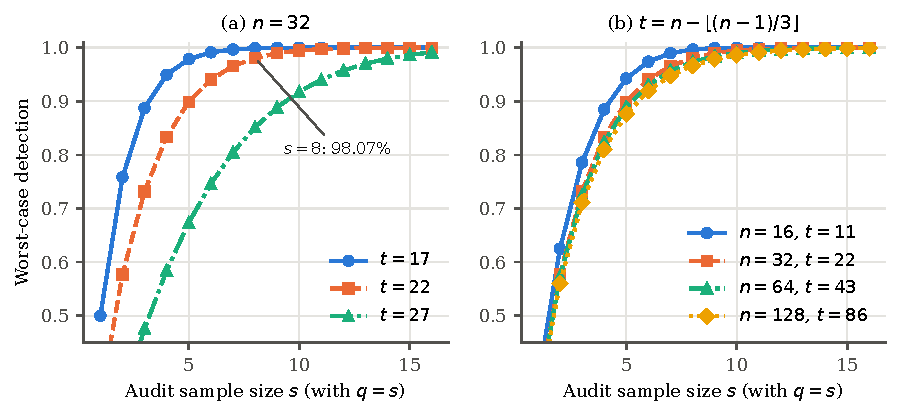
\includegraphics[width=\textwidth]{fig2_detection_vs_sample.pdf}
\caption{Exact worst-case detection $1-\binom{t-1}{s}/\binom{n}{s}$ versus sample size with $q=s$. (a)~Thresholds $t\in\{17,22,27\}$ at $n=32$; the baseline $s=8$, $t=22$ is annotated. (b)~Committee sizes 16--128 with $t=n-\lfloor(n-1)/3\rfloor$. Values for $(n,s)\in\{(16,4),(32,8),(64,12),(128,16)\}$ are listed in Table~\ref{tab:scalability}.}
\label{fig:detection}
\end{figure}

\begin{observation}[Placement cap]\label{prop:cap}
With no failures other than whole-domain outages, if every domain has at most $n-t$ custodians, no single domain outage prevents reconstruction; if some domain has more than $n-t$, its outage alone does. The cap is tight for single-domain outages.
\end{observation}

\begin{proof}
An outage of a domain of size $d$ leaves $n-d$ custodians, and $n-d\ge t$ if and only if $d\le n-t$.
\end{proof}

The baseline places four domains of eight under the cap $n-t=10$: one outage is survivable, two leave $16<22$ custodians.

\begin{observation}[Benign pass probability]\label{prop:benign}
If each custodian is independently unavailable with probability $f$ and the sample is independent of availability, the audit passes with probability $\Pr[\mathrm{Bin}(s,1-f)\ge q]$.
\end{observation}

\begin{proof}
Given the sample, its members' availability indicators are independent Bernoulli$(1-f)$, and the audit passes if and only if at least $q$ are available.
\end{proof}

The strict rule $q=s$ that maximizes detection also turns every benign miss into an alarm. For $s=q=8$ and $f=0.10$ a healthy committee passes only with probability $0.9^{8}=0.430$, although $t$ of 32 shares are reachable with probability $\Pr[\mathrm{Bin}(32,0.9)\ge 22]=0.99983$. Table~\ref{tab:acceptance} and Figure~\ref{fig:acceptance} give the trade-off. At $s=8$ no rule achieves both goals: $q=7$ lowers detection to \RAccEightSevenDet{} and raises the benign pass rate at $f=0.10$ to \RAccEightSevenPass{}. A larger sample helps: $s=16$, $q=14$ detects \RAccSixteenFourteenDet{} with benign pass rates of \RAccSixteenFourteenPassFive{} at $f=0.05$ and \RAccSixteenFourteenPassTen{} at $f=0.10$. We added this analysis after observing the alarm rate in exploratory runs and report it as design guidance, not a prespecified result.

\begin{table}[t]
\caption{Exact acceptance-rule trade-off at $n=32$, $t=22$: worst-case detection ($k=t-1$, Theorem~\ref{thm:fa}) versus the probability that a healthy committee passes under IID unavailability $f$ (Observation~\ref{prop:benign}). Post hoc analysis.}
\label{tab:acceptance}
\centering
\small
\begin{tabular}{@{}rrrrrr@{}}
\toprule
 & & Worst-case & \multicolumn{3}{c}{Benign audit pass under IID unavailability}\\
\cmidrule(lr){4-6}
$s$ & $q$ & detection & $f=0.05$ & $f=0.10$ & $f=0.20$\\
\midrule
8 & 6 & 57.5\% & 99.4\% & 96.2\% & 79.7\%\\
8 & 7 & 85.9\% & 94.3\% & 81.3\% & 50.3\%\\
8 & 8 & 98.1\% & 66.3\% & 43.0\% & 16.8\%\\
12 & 10 & 89.6\% & 98.0\% & 88.9\% & 55.8\%\\
12 & 11 & 98.2\% & 88.2\% & 65.9\% & 27.5\%\\
12 & 12 & 99.9\% & 54.0\% & 28.2\% & 6.9\%\\
16 & 13 & 93.2\% & 99.3\% & 93.2\% & 59.8\%\\
16 & 14 & 98.8\% & 95.7\% & 78.9\% & 35.2\%\\
16 & 15 & 99.9\% & 81.1\% & 51.5\% & 14.1\%\\
\bottomrule
\end{tabular}

\end{table}

\subsection{Operating characteristic and sequential audits}\label{sec:oc}

Worst-case detection hides how weak a small audit is near the threshold. Table~\ref{tab:oc} gives the full operating characteristic of Eq.~\eqref{eq:hypergeom}: with $s=q=8$ the audit accepts a committee one share short of $t$ with probability \OcEightTwentyOne{}, a live committee with no spare share with \OcEightTwentyTwo{}, and one with four spare shares with only \OcEightTwentySix{}. Only the full probe ($s=n$) separates $k=t-1$ from $k=t$ at 5\% error rates, so sampled guarantees must be stated for a safety margin $m$, testing $k\le t-1$ against $k\ge t+m$. With error rates of 5\% each, a single audit needs $s=\SepSFour$ ($q=\SepQFour$) for $m=4$, $s=\SepSSix$ ($q=\SepQSix$) for $m=6$ and $s=\SepSEight$ ($q=\SepQEight$) for $m=8$. A sequential probability ratio test across audits\cite{wald1945sprt}, valid under the static state of Corollary~\ref{cor:repeat}, is far cheaper: for $m=6$ it decides on average after \AsnSixteenDead{} audits for a failed committee and \AsnSixteenLive{} for a live one with $s=16$, $q=14$, and after \AsnEightDead{} and \AsnEightLive{} with $s=q=8$ (Wald's approximations). Audits should therefore be specified by the margin they certify and the error rates they achieve, not by worst-case detection. This analysis is exact.

\begin{table}[t]
\caption{Exact operating characteristic: probability that an audit with sample size $s$ and threshold $q$ accepts when $k$ of $n=32$ custodians are ready ($t=22$, uniform sampling, Theorem~\ref{thm:fa}).}
\label{tab:oc}
\centering
\small
\begin{tabular}{@{}rrrrrrrr@{}}
\toprule
 & & \multicolumn{6}{c}{Pr[audit accepts] with $k$ ready custodians ($n=32$, $t=22$)}\\
\cmidrule(lr){3-8}
$s$ & $q$ & $k=21$ & $k=22$ & $k=24$ & $k=26$ & $k=28$ & $k=30$\\
\midrule
8 & 8 & 1.9\% & 3.0\% & 7.0\% & 14.9\% & 29.5\% & 55.6\%\\
8 & 7 & 14.1\% & 19.3\% & 33.3\% & 52.4\% & 74.6\% & 94.4\%\\
16 & 14 & 1.2\% & 2.7\% & 11.0\% & 32.7\% & 70.0\% & 100.0\%\\
16 & 13 & 6.8\% & 12.6\% & 34.3\% & 67.3\% & 94.9\% & 100.0\%\\
24 & 20 & 0.1\% & 0.5\% & 8.2\% & 47.6\% & 100.0\% & 100.0\%\\
\bottomrule
\end{tabular}

\end{table}

\begin{proposition}[Deadline budget]\label{prop:budget}
Under Assumptions~\ref{as:board} and~\ref{as:sync}, suppose at least $t$ custodians are non-faulty, hold their shares and follow the protocol, and the combiner is work-conserving, verifies serially and verifies each authenticated index at most once. Then a dispute requested at $\tau$ obtains $t$ valid partials by $\tau+\delta_b+c_p+\delta+n\,c_v$, and the key is recovered $c_c$ later. Hence $\Delta_d\ge\delta_b+c_p+\delta+n\,c_v$ suffices for $\DDL$, and $n\,c_v$ may be replaced by $t\,c_v$ if no invalid response precedes the $t$-th valid one.
\end{proposition}

\begin{proof}
Each of the $t$ correct custodians sees the request by $\tau+\delta_b$ and its response arrives by $T=\tau+\delta_b+c_p+\delta$. Authenticated channels prevent an adversary from occupying a correct custodian's index, so the combiner verifies at most one response per index, at most $n$ in total, and never idles while responses are pending; it therefore finishes by $T+n\,c_v$, or by $T+t\,c_v$ if no invalid response comes first.
\end{proof}

On a production settlement layer, $\delta_b$ is a block or finality time and can dominate; in our testbed $\delta_b$ is negligible and unoptimized verification makes $t\,c_v$ the largest term.

% =====================================================================
\section{Evaluation}\label{sec:evaluation}

We compare the audit with simpler checks (Q1), separate audit outcomes from dispute success under failures (Q2), identify what governs dispute completion (Q3), and measure scaling (Q4).

\paragraph{Method.} Table~\ref{tab:config} lists every experiment, and each result carries one of four evidence labels. \emph{Exact} values are closed form under a declared model. \emph{Simulation} results come from three cells whose parameters, endpoints and seeds were fixed and hashed before execution; each has 131{,}072 draws, above the 73{,}778 that Hoeffding's inequality requires for a half-width of 0.005 at 95\% confidence\cite{hoeffding1963}. Where an exact value exists, the cells serve as an implementation check against it. The sampling-policy cell compares uniform and stratified samples on common random numbers. \emph{Microbenchmarks} are single-process medians, and \emph{emulation} runs 32 custodian processes on one host. Proportions carry 95\% Wilson intervals\cite{wilson1927}.

\begin{table}[t]
\caption{Experimental configuration. The baseline committee is $n=32$, $t=22$, $s=q=8$ with four failure domains of eight custodians.}
\label{tab:config}
\centering
\footnotesize
\begin{tabularx}{\textwidth}{@{}>{\raggedright\arraybackslash}p{0.2\textwidth}>{\raggedright\arraybackslash}p{0.3\textwidth}X@{}}
\toprule
Experiment family & Parameters & Execution and evidence label\\
\midrule
Static bound (Eq.~\ref{eq:bound}) & $n\in\{16,32,64,128\}$, $t=n-\lfloor (n-1)/3\rfloor$, $s\in\{1,\dots,16\}$, $q=s$; baseline $n=32,t=22,s=q=8$ & Exact closed form\\
Simulation cells & $n=32,t=22,s=q=8$, 4 domains of 8. IID: $p_{\mathrm{off}}=0.10$. STRAT: $p_{\mathrm{dom}}=0.20$, $p_{\mathrm{off}}=0.02$, uniform vs.\ 2-per-domain quota. SW: $w=11$ & 32 seed blocks $\times$ 4{,}096 draws $=131{,}072$ per cell; seeds frozen before execution; simulation\\
Correlation model & $f\in\{0,0.025,\dots,0.40\}$; IID vs.\ 2/4/8 equal domains & Exact; declared synthetic model\\
Acceptance rule & $s\in\{8,12,16\}$, $q\in[\lceil s/2\rceil,s]$, IID $f\in\{0.05,0.10,0.20\}$ & Exact; post hoc\\
Cryptographic cost & ffdhe2048, ffdhe3072 (RFC 7919) and the 256-bit prototype group; $n\le 128$ & Local microbenchmark, CPython 3.13, Apple M4 Pro\\
Deadline testbed & ffdhe2048, $n=32,t=22$; 8 profiles $\times$ 300 traces; one-way delay lognormal (median 0/40/120\,ms); 2\% loss; 10 or 11 crashes; one-domain outage; $\Delta_d\in\{0.25,0.5,1,2,5\}$\,s & 32 custodian processes on one host, loopback TCP, real cryptography; emulation\\
\bottomrule
\end{tabularx}

\end{table}

\subsection{Readiness baselines (Q1)}

Table~\ref{tab:baselines} compares the canary audit with the obvious alternatives. A heartbeat is answered even by a custodian that lost its share, registration is checked once, and decrypting a real record discloses it. A full-committee canary probe detects every static catastrophic state at four times KEYSTONE's per-round cost; it is the case $s=n$ of Theorem~\ref{thm:fa} and is affordable for one audit per epoch at $n=32$. Sampling pays off when audits are frequent, committees are large or responses are recorded on chain: at the measured 57{,}882 gas per response (Table~\ref{tab:gas}), recording responses costs about $0.46$ million gas per audit for $s=8$ and $1.85$ million for $s=32$.

\begin{table}[t]
\caption{Readiness checks compared. Costs are measured medians for ffdhe2048 in the prototype (Table~\ref{tab:operations}); bytes are canonical request plus response transcripts.}
\label{tab:baselines}
\centering
\footnotesize
\begin{tabularx}{\textwidth}{@{}>{\raggedright\arraybackslash}p{0.17\textwidth}>{\raggedright\arraybackslash}p{0.15\textwidth}>{\raggedright\arraybackslash}p{0.14\textwidth}>{\raggedright\arraybackslash}p{0.17\textwidth}X@{}}
\toprule
Readiness check & Exercises the secret share? & Touches production ciphertext? & Detects a static state with $k=t-1$ ready shares & Cost per check ($n=32$, ffdhe2048, measured)\\
\midrule
Liveness heartbeat & No & No & No: a node that lost its share still answers & 1 message per node; no group operations\\
Share registration (Feldman/PVSS check) & Once, at setup & No & No: says nothing about later share loss & One-time $O(nt)$ exponentiations at epoch setup\\
Full-committee canary probe & Yes & No (canary) & Yes, with probability 1 & 32 proofs + 32 verifications; 8501\,ms CPU; 36,991\,B\\
KEYSTONE sampled canary ($s=q=8$) & Yes, for the sampled members & No (canary) & Yes, with probability 0.9807 (Eq.~\ref{eq:bound}) & 8 proofs + 8 verifications; 2125\,ms CPU; 9,415\,B\\
Decrypt a real record as a test & Yes & Yes: exposes a production record & Yes & $t$ verifications plus a real disclosure; excluded by design\\
\bottomrule
\end{tabularx}

\end{table}

\subsection{Robustness under failures (Q2)}\label{sec:eval-robust}

In the simulation cells (Table~\ref{tab:robustness}), 10\% independent unavailability leaves the committee reconstructable in \RIIDRecon{} of draws while the strict audit passes in only \RIIDAudit{}: it is a sensitive alarm, not a health score, as Observation~\ref{prop:benign} predicts. Under 20\% domain outages, stratified sampling raised conditional detection of catastrophic draws from \RStratDetU{} to \RStratDetS{} and lowered the benign pass rate from \RStratPassU{} to \RStratPassS{}. The prespecified endpoint, the paired difference in detected catastrophes per draw, was \RStratD{} with Hoeffding half-width \RStratHW{}, a conservative test that cannot resolve an effect this small; a post hoc exact sign test on the \RStratDiscordant{} discordant pairs, all favoring stratification, gives $p=\McNemarP$, and Proposition~\ref{prop:strat} gives the exact difference for any placement. With eleven selective withholders, audits passed in \RSWAudit{} of draws and disputes succeeded in \RSWDispute{}; this cell instantiates the deterministic witness of Observation~\ref{prop:nonimpl}(2) and only confirms that the implementation reproduces it.

\begin{table}[t]
\caption{Simulation cells, 131{,}072 draws each, 95\% Wilson intervals. Reconstructable means at least $t$ custodians can serve the dispute.}
\label{tab:robustness}
\centering
\footnotesize
\begin{tabular}{@{}lrr@{}}
\toprule
Scenario & Audit pass & Reconstructable\\
\midrule
IID 10\% unavailable & 43.1\% [42.8, 43.3] & 99.98\% [99.97, 99.99]\\
Domain outage 20\%, uniform sample & 37.3\% [37.0, 37.6] & 81.3\% [81.1, 81.6]\\
Domain outage 20\%, stratified sample & 34.9\% [34.7, 35.2] & 81.3\% [81.1, 81.6]\\
11 selective withholders & 100.0\% [99.997, 100.000] & 0.0\% [0.000, 0.003]\\
\bottomrule
\end{tabular}

\end{table}

Placement matters more (Figure~\ref{fig:correlation}). At per-unit unavailability $f=0.10$, an IID committee reconstructs with probability \RIIDReconTen{}, four domains of eight (under the cap of Observation~\ref{prop:cap}) with \RDomFourRecon{}, and two domains of sixteen, which violate it, with only \RDomTwoRecon{}. These values are exact under a declared synthetic model; field studies show that correlated failures dominate real unavailability\cite{ford2010availability}.

\begin{figure}[t]
\centering
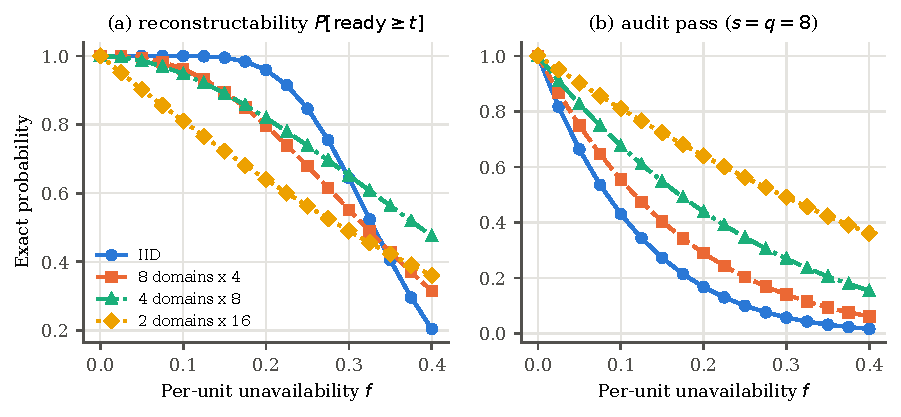
\includegraphics[width=\textwidth]{fig4_iid_vs_correlated.pdf}
\caption{IID versus domain-correlated unavailability at $n=32$, $t=22$. A domain fails with probability $f$ and takes all its members; in the IID model each custodian fails independently with probability $f$. (a)~Reconstructability. (b)~Audit pass with $s=q=8$. Exact; a 20{,}000-draw Monte Carlo check agrees within $0.009$.}
\label{fig:correlation}
\end{figure}

\begin{figure}[t]
\centering
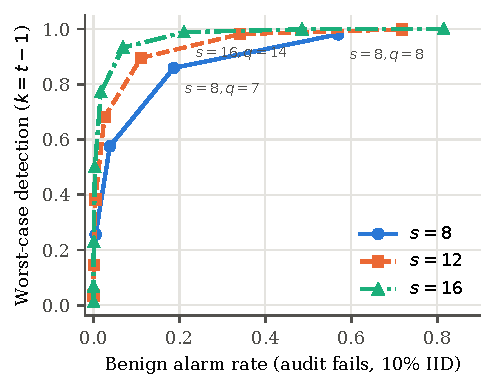
\includegraphics[width=0.62\textwidth]{fig6_acceptance_tradeoff.pdf}
\caption{Detection versus benign alarm rate (the audit fails while the committee is healthy, $f=0.10$) for each $q$, one curve per sample size. Exact values from Table~\ref{tab:acceptance} and its full source grid.}
\label{fig:acceptance}
\end{figure}

\subsection{Deadline liveness in an emulated testbed (Q3)}\label{sec:eval-deadline}

Thirty-two custodian processes, each an asyncio TCP server holding only its own ffdhe2048 share, and one combiner run on one host. Each trace runs one canary audit and one dispute over a freshly sealed 1\,KiB record; the combiner verifies proofs on arrival, stops at $t=22$ valid partials, combines, unwraps $K_r$ and checks the plaintext. One-way delays are lognormal with the profile's median, loss drops messages without retransmission, and crashed custodians never answer. Each of eight profiles ran \RDLTraces{} traces with seeds fixed in advance.

Table~\ref{tab:testbed} gives the results. No dispute finished in under 3.5\,s, so the primary endpoint fixed before the run, success by $\Delta_d=2$\,s, was $0\%$ in every profile; that deadline was set without budgeting for the serial verification term of Proposition~\ref{prop:budget}, which in this prototype alone exceeds 2\,s. Within 5\,s every reconstructable dispute succeeded except one control trace (299 of 300), with medians from \RDLMedLo{} to \RDLMedHi\,s and a slowest success of \RDLMaxSucc\,s; that trace timed out with 19 valid partials during unrelated load on the shared host. Without injected delay the median was \RDLControlMed\,ms, of which 22 serial verifications at \RVerifyTwoK\,ms (Table~\ref{tab:operations}) account for about 2{,}980\,ms; the remainder was not instrumented. A 120\,ms-median delay moved the median only to \RDLGlobalMed\,ms, because responses arrive while earlier ones are still being verified, and a heavy-tailed law ($\sigma=1.2$) did not lengthen completion (95th percentile \RDLHeavyTailPninefive\,ms). Ten crashes and a domain outage finished slightly faster, plausibly because fewer processes competed for the CPU; eleven crashes defeated every dispute (\RDLCrashElevenSucc{} succeeded), since $21<t$ custodians remain. In this unoptimized single-host setting, completion was bounded by computation rather than emulated network delay; we did not measure optimized or batched verification.

\begin{table}[t]
\caption{Emulated testbed, 32 custodian processes on one host with real ffdhe2048 cryptography, \RDLTraces{} traces per profile, 95\% Wilson intervals. Audit pass is $q=8$ valid responses within the 6\,s timeout; dispute columns require the correct plaintext by the stated deadline; times are over successful disputes.}
\label{tab:testbed}
\centering
\footnotesize
\begin{tabular}{@{}lrrrrr@{}}
\toprule
Profile & Audit pass & By $\Delta_d=2$\,s & By 5\,s & Median & p95\\
\midrule
control & 100.0\% [98.7, 100.0] & 0.0\% [0.0, 1.3] & 99.7\% & 3818\,ms & 3936\,ms\\
regional & 100.0\% [98.7, 100.0] & 0.0\% [0.0, 1.3] & 100.0\% & 3841\,ms & 3908\,ms\\
global & 100.0\% [98.7, 100.0] & 0.0\% [0.0, 1.3] & 100.0\% & 3875\,ms & 4016\,ms\\
global loss2 & 71.7\% [66.3, 76.5] & 0.0\% [0.0, 1.3] & 100.0\% & 3829\,ms & 3886\,ms\\
global crash10 & 2.3\% [1.1, 4.7] & 0.0\% [0.0, 1.3] & 100.0\% & 3692\,ms & 3775\,ms\\
global crash11 & 1.7\% [0.7, 3.8] & 0.0\% [0.0, 1.3] & 0.0\% & -- & --\\
global domain outage & 5.7\% [3.6, 8.9] & 0.0\% [0.0, 1.3] & 100.0\% & 3700\,ms & 3780\,ms\\
heavy tail & 98.3\% [96.2, 99.3] & 0.0\% [0.0, 1.3] & 100.0\% & 3772\,ms & 3850\,ms\\
\bottomrule
\end{tabular}

\end{table}

Audit pass rates on real cryptography matched the exact expectations (Eq.~\eqref{eq:hypergeom} for crashes and outages, Observation~\ref{prop:benign} for loss): \RDLCrashTenAudit{} against \RExpCrashTen{} with ten crashes, \RDLDomainOutAudit{} against \RExpDomainOut{} with one domain down, and \RDLLossAudit{} against \RExpLoss{} with 2\% loss, while the dispute succeeded in every trace of these profiles. A single audit took \RDLAuditMedLo--\RDLAuditMedHi\,s at the median. Under the heavy-tailed law the audit failed in 5 of 300 traces, each with 7 of 8 responses verified before the 6\,s timeout, consistent with the lognormal tail.

\subsection{Performance and scalability (Q4)}

Table~\ref{tab:operations} gives per-operation costs of the pure-Python prototype; optimized libraries, in particular elliptic-curve groups, are substantially faster. At ffdhe2048 a partial decryption with proof takes \RProveTwoK\,ms and its verification \RVerifyTwoK\,ms, and verifying 22 partials and combining takes \RCombineTwoK\,ms (\RCombineThreeK\,ms at ffdhe3072). The 256-bit group is listed for reference only and is not a secure size. Audit cost grows with $s$ and dispute cost with $t$ (Table~\ref{tab:scalability}); Table~\ref{tab:gas} gives gas costs.

\begin{table}[t]
\caption{Median wall time per operation, CPython 3.13 on an Apple M4 Pro; RFC~7919 groups\cite{rfc7919} with $\ell=(p-1)/2$ and generator~4. Pure-Python reference implementation.}
\label{tab:operations}
\centering
\small
\begin{tabular}{@{}lrrr@{}}
\toprule
Operation (median, ms) & 256-bit prototype & ffdhe2048 & ffdhe3072\\
\midrule
Canary derivation $H_G$ & 0.08 & 16.99 & 54.32\\
Partial decryption + DLEQ proof & 0.58 & 130.30 & 420.54\\
DLEQ verification & 0.75 & 135.36 & 430.58\\
Seal 1\,KiB record & 0.22 & 48.32 & 156.48\\
Partial response size (bytes) & 253 & 1149 & 1661\\
\bottomrule
\end{tabular}

\end{table}

\begin{table}[t]
\caption{Scalability with $t=n-\lfloor(n-1)/3\rfloor$. Detection is exact (Eq.~\eqref{eq:bound}, $q=s$). Audit CPU is $s$ proofs plus $s$ verifications; bytes are one request plus $s$ responses. Dispute time is measured verification of $t$ partials plus combination.}
\label{tab:scalability}
\centering
\small
\begin{tabular}{@{}rrrrrrrr@{}}
\toprule
 & & & & \multicolumn{2}{c}{Audit, ffdhe2048} & \multicolumn{2}{c}{Dispute: verify $t$ + combine}\\
\cmidrule(lr){5-6}\cmidrule(lr){7-8}
$n$ & $t$ & $s$ & Detection & CPU & Bytes & ffdhe2048 & ffdhe3072\\
\midrule
16 & 11 & 4 & 88.46\% & 1063\,ms & 4,819 & 1585\,ms & 5040\,ms\\
32 & 22 & 8 & 98.07\% & 2125\,ms & 9,415 & 3213\,ms & 10201\,ms\\
64 & 43 & 12 & 99.66\% & 3188\,ms & 14,011 & 6230\,ms & 20086\,ms\\
128 & 86 & 16 & 99.92\% & 4250\,ms & 18,607 & 12534\,ms & 40201\,ms\\
\bottomrule
\end{tabular}

\end{table}

\begin{table}[t]
\caption{Bulletin-board gas per operation, measured with Foundry 1.5.1 and Solidity 0.8.24 (test-body gas; fixture setup excluded), in the small harness committee named in the scope column; values are deterministic.}
\label{tab:gas}
\centering
\footnotesize
\begin{tabularx}{\textwidth}{@{}l r X@{}}
\toprule
Bulletin-board operation & Gas & Harness scope\\
\midrule
Register epoch & 223,629 & n=5, t=3; duplicate-identity validation enabled\\
Open audit & 125,107 & three sampled members; q=3\\
Submit audit response & 57,882 & first commitment from one sampled custodian\\
Mark invalid response & 27,704 & admin records a non-zero evidence hash\\
Record equivocation & 51,710 & second conflicting commitment from one custodian\\
Finalize audit & 29,142 & two responses for a three-member sample after deadline\\
Open dispute & 144,149 & n=5, t=3; all members eligible\\
Cancel request & 5,709 & admin cancels one open audit\\
\bottomrule
\end{tabularx}

\end{table}

% =====================================================================
\section{Discussion}\label{sec:discussion}

Availability is layered: data availability concerns encrypted bytes, share registration the key's formation, a readiness audit present share access, and a dispute whether $t$ custodians serve a specific target in time; the evaluation separates each layer.

Four design consequences follow. First, specify audits by the safety margin they certify: choose $s$ and $q$, or a sequential test across audits, for target error rates at $k\le t-1$ and $k\ge t+m$ (Section~\ref{sec:oc}), which favors larger samples with $q<s$. Second, placement under the cap $n-t$ matters more than the sampling policy. Third, deadlines must budget for the ledger delay and for verifying up to $n$ proofs, or $t$ when no invalid response comes first (Proposition~\ref{prop:budget}); optimized or batched verification is the first improvement. Fourth, if untrusted parties can obtain releases, the dispute path must bind each release to its record (Proposition~\ref{prop:malleable}).

Invalid proofs and equivocation are transferable evidence, whereas non-response proves only absence and its attribution depends on timing\cite{lewis2025accountable}, so slashing should be reserved for transferable evidence. Finally, the audit cannot detect selective withholding, because canaries are unrelated to records by design (Lemma~\ref{lem:sim}). Making canaries indistinguishable from record components would stop observers from checking that an audit opened no production record (Lemma~\ref{lem:subst}), so resistance needs a different mechanism, such as unpredictable dispute routing or economic commitments enforced by the deadline transcript.

% =====================================================================
\section{Related work}\label{sec:related}

Table~\ref{tab:related} summarizes how KEYSTONE relates to other checks of availability or readiness.

\begin{table}[t]
\caption{Mechanisms that check some form of availability or readiness. ``Secret-key operation'' means the check makes a custodian apply its secret share. Entries describe the mechanism class, not every system in it.}
\label{tab:related}
\centering
\footnotesize
\begin{tabularx}{\textwidth}{@{}>{\raggedright\arraybackslash}p{0.27\textwidth}>{\raggedright\arraybackslash}X>{\raggedright\arraybackslash}p{0.17\textwidth}>{\raggedright\arraybackslash}p{0.17\textwidth}@{}}
\toprule
Mechanism & What is checked & Secret-key operation & Deadline evidence\\
\midrule
Liveness heartbeat & A process answers & No & No\\
Threshold-wallet heartbeat (tBTC v2)\cite{tbtc2026heartbeat} & The full signing group signs a heartbeat message & Yes (signing) & A failed heartbeat triggers fund migration\\
Proof of custody\cite{feist2021custody} & A validator holds the data it attests to & Secret-dependent bit & Challenge and penalty\\
PoR and PDP\cite{juels2007por,ateniese2007pdp,bowers2009hail} & A server still stores a file & No & No\\
Data-availability sampling\cite{albassam2021fraud,hallandersen2025das,eip7594} & Published data are retrievable & No & No\\
VSS, PVSS and DKG transcripts\cite{feldman1987vss,schoenmakers1999pvss,gennaro2007dkg} & Shares were distributed consistently & At setup only & No\\
Threshold-release systems\cite{kokoriskogias2020calypso,stengele2021ethtid,bebel2022ferveo} & A release is performed when requested & At release only & System-specific\\
KEYSTONE & $q$ of $s$ sampled custodians can apply their shares now; $t$ custodians serve a dispute by $\Delta_d$ & Before release (canary) and at release & Bulletin board\\
\bottomrule
\end{tabularx}
\end{table}

\paragraph{Optimistic and verifiable computation.} Optimistic rollups rely on dispute protocols in which an honest challenger forces correct results on chain\cite{kalodner2018arbitrum}; opML applies this to machine-learning inference\cite{conway2024opml}, and EigenAI re-executes private inference in a trusted environment after a threshold key release\cite{eigenai2026}. These systems assume the challenger can read the disputed inputs. With encrypted inputs that assumption becomes the requirement that keys be serviceable before the deadline, which KEYSTONE isolates and audits without changing the dispute game.

\paragraph{Threshold decryption and key management.} Threshold cryptosystems\cite{desmedt1990threshold}, their chosen-ciphertext-secure variants with verifiable shares\cite{shoup2002securing} and DLEQ proofs\cite{chaum1992dleq,fiat1987prove} provide the release mechanism. Verifiable and publicly verifiable secret sharing and distributed key generation\cite{feldman1987vss,schoenmakers1999pvss,gennaro2007dkg,das2022adkg} make shares consistent when created, and proactive and dynamic sharing refreshes them\cite{herzberg1995proactive,yurek2023dpss}. A refresh, including dynamic-committee resharing\cite{maram2019churp}, also exercises every share, but it is infrequent and costly, and shares can be lost between refreshes. A canary response is structurally a threshold-coin share\cite{cachin2005constantinople} or a threshold-signature share on a hashed message\cite{boldyreva2003threshold}; our contribution is not this primitive but its use as a sampled readiness test, with the properties it can and cannot certify. Context-dependent threshold decryption isolates shares across contexts\cite{boneh2025context}. KEYSTONE uses these primitives unchanged and asks whether enough custodians can apply their shares \emph{now}.

\paragraph{Threshold release on ledgers.} CALYPSO releases on-ledger secrets to authorized readers through a threshold committee with an auditable access log\cite{kokoriskogias2020calypso}, and ETHTID provides threshold disclosure on Ethereum\cite{stengele2021ethtid}. Encrypted mempools face the same operational concerns of committees, epochs, collusion and timely decryption\cite{bebel2022ferveo,bormet2025epochless,choudhuri2024mempool}. FairBlock applies identity-based encryption so that a committee exchanges a fixed number of decryption shares per block, independent of the number of transactions\cite{momeni2023fairblock}, and F3B, building on CALYPSO, has a secret-management committee release a per-transaction key once the transaction is finalized\cite{zhang2023f3b}. In both, timely decryption depends on a threshold of committee members serving the release, which is the property DKA makes explicit; the published descriptions we found specify the release path but no pre-release readiness audit. UQ-Vote combines a consensus-finalized bulletin board with consensus-authorized threshold decryption and evaluates liveness under faults\cite{liu2026uqvote}. Authorization by finalized state, public request logs and decryption deadlines are thus established, and we do not claim them. These systems specify the release path; KEYSTONE adds the deadline-bound property that release must satisfy for disputes, a pre-release audit that measures it without opening records, and an analysis of what passing it implies.

\paragraph{Proofs of storage, custody and heartbeats.} Proofs of retrievability and provable data possession spot-check random parts of a stored file and bound the probability that a server missing data passes\cite{juels2007por,ateniese2007pdp}; HAIL extends this to servers under a mobile adversary\cite{bowers2009hail}. KEYSTONE's audit belongs to this family: the DLEQ proof is a proof of knowledge (Lemma~\ref{lem:correct}), and Theorem~\ref{thm:fa} plays the role of their sampling bounds. It differs in that possession is not service, a gap KEYSTONE makes explicit (Observation~\ref{prop:nonimpl}); in that confidentiality forces canary responses to be useless for decrypting records (Lemmas~\ref{lem:sim} and~\ref{lem:subst}); and in that DKA is a multi-party, threshold, target-specific and deadline-bound property. Proof-of-custody proposals make validators commit to a secret-dependent bit of attested data so lazy validators can be penalized\cite{feist2021custody}. The closest deployed analogue is the tBTC v2 heartbeat, in which each threshold wallet's signing group signs periodic messages and funds leave a wallet that fails one\cite{tbtc2026heartbeat}; KEYSTONE instead samples custodians with exact operating characteristics, audits decryption shares under a confidentiality constraint, and ties readiness to dispute deadlines. Data-availability proofs and sampling\cite{albassam2021fraud,hallandersen2025das,eip7594} concern public data, which KEYSTONE takes as given.

\paragraph{Accountability.} Slashing conditions\cite{buterin2017casper} and BFT forensics\cite{sheng2021forensics} attribute safety violations with transferable evidence, threshold traitor tracing addresses coalitions that leak decryption capability\cite{boneh2023accountability}, and attributing liveness failures depends on timing\cite{lewis2025accountable}.

% =====================================================================
\section{Threats to validity and limitations}\label{sec:validity}

\paragraph{Novelty.} The components are not new; our claim covers the property decomposition, the confidentiality-preserving audit and its analysis, and the labeled evaluation, and it rests on a bounded literature search.

\paragraph{Internal validity.} The simulation design was hashed before execution, but the hash is self-recorded and the design was not reviewed by an independent party; the acceptance-rule and operating-characteristic analyses were added afterwards. The testbed shares one CPU among 33 processes, which explains the slightly faster crash profiles and the one control timeout; both are reported, not discarded.

\paragraph{Construct and external validity.} The audit measures present sampled serviceability, not future cooperation, and repeated-audit bounds need a static or modeled readiness process. Failure models are synthetic, the testbed uses loopback TCP with synthetic delays, geo-distributed effects and clock skew are not measured, and timings reflect pure Python.

\paragraph{Prototype scope.} A dealer replaces distributed key generation; the plain KEM provides $\PAC$ but not $\PAC^{+}$; the contract trusts an administrator for sampling, invalid-response evidence and cancellation; neither code nor contract has been externally audited; and the lemmas hold in the random-oracle model with static corruption.

% =====================================================================
\section{Conclusion and future directions}\label{sec:conclusion}

Ciphertext availability does not ensure that the threshold service needed for an encrypted-rollup dispute answers in time. We defined dispute-key availability and the weaker properties it is confused with, showed that a beacon-derived canary audit exercises real shares while its transcripts are simulatable from public data, gave its exact operating characteristics, the sample sizes and sequential tests that certify a safety margin, a placement condition and a deadline budget, and showed that confidentiality against parties who obtain other releases requires binding releases to records. The evaluation confirmed each separation: a small strict audit barely distinguishes a failed committee from a live one and alarms often on healthy committees, selective withholders pass every audit and defeat every dispute, and in the emulated committee all but one reconstructable dispute completed within five seconds, bounded by serial proof verification in our unoptimized prototype. Future work should address selective withholding, which the audit provably cannot detect alone; temporal readiness models calibrated on operational data; and a production instantiation with distributed key generation, record-bound releases, optimized verification and realistic ledger delays, evaluated across regions.

% =====================================================================
\section*{Statements and Declarations}

\paragraph*{Ethical considerations.}This article reports non-human computational research using synthetic data, simulation, locally generated prototype outputs and smart-contract tests. It involves no human participants, personal data, production secrets or live systems, so ethical approval was not required.

\paragraph*{Consent to participate.}Not applicable.

\paragraph*{Consent for publication.}Not applicable.

\paragraph*{Declaration of conflicting interest.}The author(s) declared no potential conflicts of interest with respect to the research, authorship and/or publication of this article.

\paragraph*{Funding statement.}The author(s) received no financial support for the research, authorship and/or publication of this article.

\paragraph*{Data availability.}Source code, frozen designs with SHA-256 hashes, seed schedules, raw per-block and per-trace outputs, and the scripts that generate every table, figure and in-text number are provided as anonymized supplementary material for review. A public repository link is given on the title page and will be included in the published article.

\paragraph*{Declaration of AI use.}AI assistance was used for drafting text, integrating code, scripting experiments and generating figures. The author(s) verified the scientific content, the proofs and every reported number against the generated outputs, and take full responsibility for the article.

\bibliographystyle{unsrtnat}
\bibliography{references}

\end{document}
